%\section{Determination of non-equilibrium cross-section of IMF in p + Ag reaction at 480 MeV}
\section{Introduction}
In chapter \ref{chapter:4} the predictive capabilities of the different spallation models describing the first stage of reaction were tested with a new measured data set for production of $p$, $d$, $t$, $\pi^{+}$ and $\pi^{-}$ in reaction of $p$+$Nb$. 
 
In chapter \ref{chapter:5} the models of de-excitation of products of the first stage of reaction are validated. It is done by means of  
simulations of the isotopic total production cross-section of IMF and heavier residues of atomic number from Z = 3 to Z = 56. They were  produced in the reaction of $^{136}Xe$+$p$ at $Xe$ beam energy of 1 GeV/nucleon.

In all the above studies a two-step mechanism of the reactions was postulated.  The first stage of the collisions proceeded as non-equilibrium process - cascade of nucleon-nucleon and nucleon-pion interactions which lead to a single, equilibrated but excited heavy remnant nucleus.  
This nucleus in the second stage of the process could evaporate nucleons, light and heavy particles and could as well undergo the fission or (multi-)fragmentation.  

As it was described in the previous section, such scenario of the reaction was able to reproduce the main properties of the mass dependence of total isotopic cross-sections. 

Furthermore, two specific observations might be done as concerns models of the second step of the reaction: \\
(i) the best  reproduction of the data is 
assured by GEMINI++ model, and \\
(ii) the GEMINI++ is the only model which provides the cross-sections values not overestimating the experimental ones. 

Very similar observations were published in  \cite{sharma2016ranking} after investigation of huge set of experimental data for $p$+$Ag$ collisions at beam energy of 480 MeV,
measured by Green et al.\cite{Green1984}.

The first observation may lead to the conclusion, that the mechanism realized in GEMINI++ is the closest to reality. The second observation may indicate that some additional mechanisms besides the equilibrium processes are necessary in the second stage of the spallation reaction.  

Such non-equilibrium processes were indeed observed in proton induced spallation on many target nuclei starting from Al  \cite{fidelus2014sequential} , Ni  \cite{budzanowski2009variation}, to Ag  \cite{fidelus2017non} and Au  \cite{budzanowski2010comparison}.  

Unfortunately, no microscopic models of such processes exist. Thus, the observed phenomena were described by phenomenological models of moving source which parameters must be adjusted to the experimental double differential  cross-sections $d^2\sigma/d\Omega dE$.  

In the present chapter the extension of the studies described in the previous chapters is proposed. It consists in supplementing of the microscopic contributions realized by INCL++
(for the first stage of reaction) and GEMINI++ (for the second stage of the process) by the phenomenological moving source contribution.  
The properties of moving source are determined from the fit to the experimental double differential cross-sections $d^2\sigma/d\Omega dE$ of $p$+$Ag$ collisions at 480 MeV proton energy, provided by \cite{Green1984}.  

The main motivation of this chapter is to further investigate the same data in order to search for the missing contribution of the possible processes, understand their nature and their dependence on the properties of the emitted particles in terms of A, Z and the third component of the isospin T$_3$. 

To achieve this goal, it is of utmost importance to calculate the total production cross-section of the IMF with possibility to extract the contribution of the non-equilibrium stage. 

In the experiment of Green \emph{et al.} \cite{Green1984}, the double differential cross-sections (d$^2\sigma$/d$\Omega$dE) were measured for different scattering angles ranging from 10$^{\circ}$ to 160$^{\circ}$. The differential cross-section has a smooth energy and angle dependence, so interpolation and extrapolation of the cross-sections for different emission angles were performed in order to determine the total cross-section.
%%%
%%%
\section{Extracting the experimental total production cross-sections}\label{totalprod}

 The source of missing mechanism and its contribution to the total cross-section can be evaluated using the phenomenological models. To reconstruct the total production cross-section from experimental data, the simulated cross-section values of GEMINI++  ($d^2\sigma/dEd\Omega$) were supplied by incoherent addition of isotropic emission from highly excited Maxwellian source (or two sources) moving along the beam direction.
 
%%%%%% Combining chapter 6 and 7 - 
%\begin{figure*}
\begin{figure}[!h]
	% Requires \usepackage{graphicx}
	\centering
		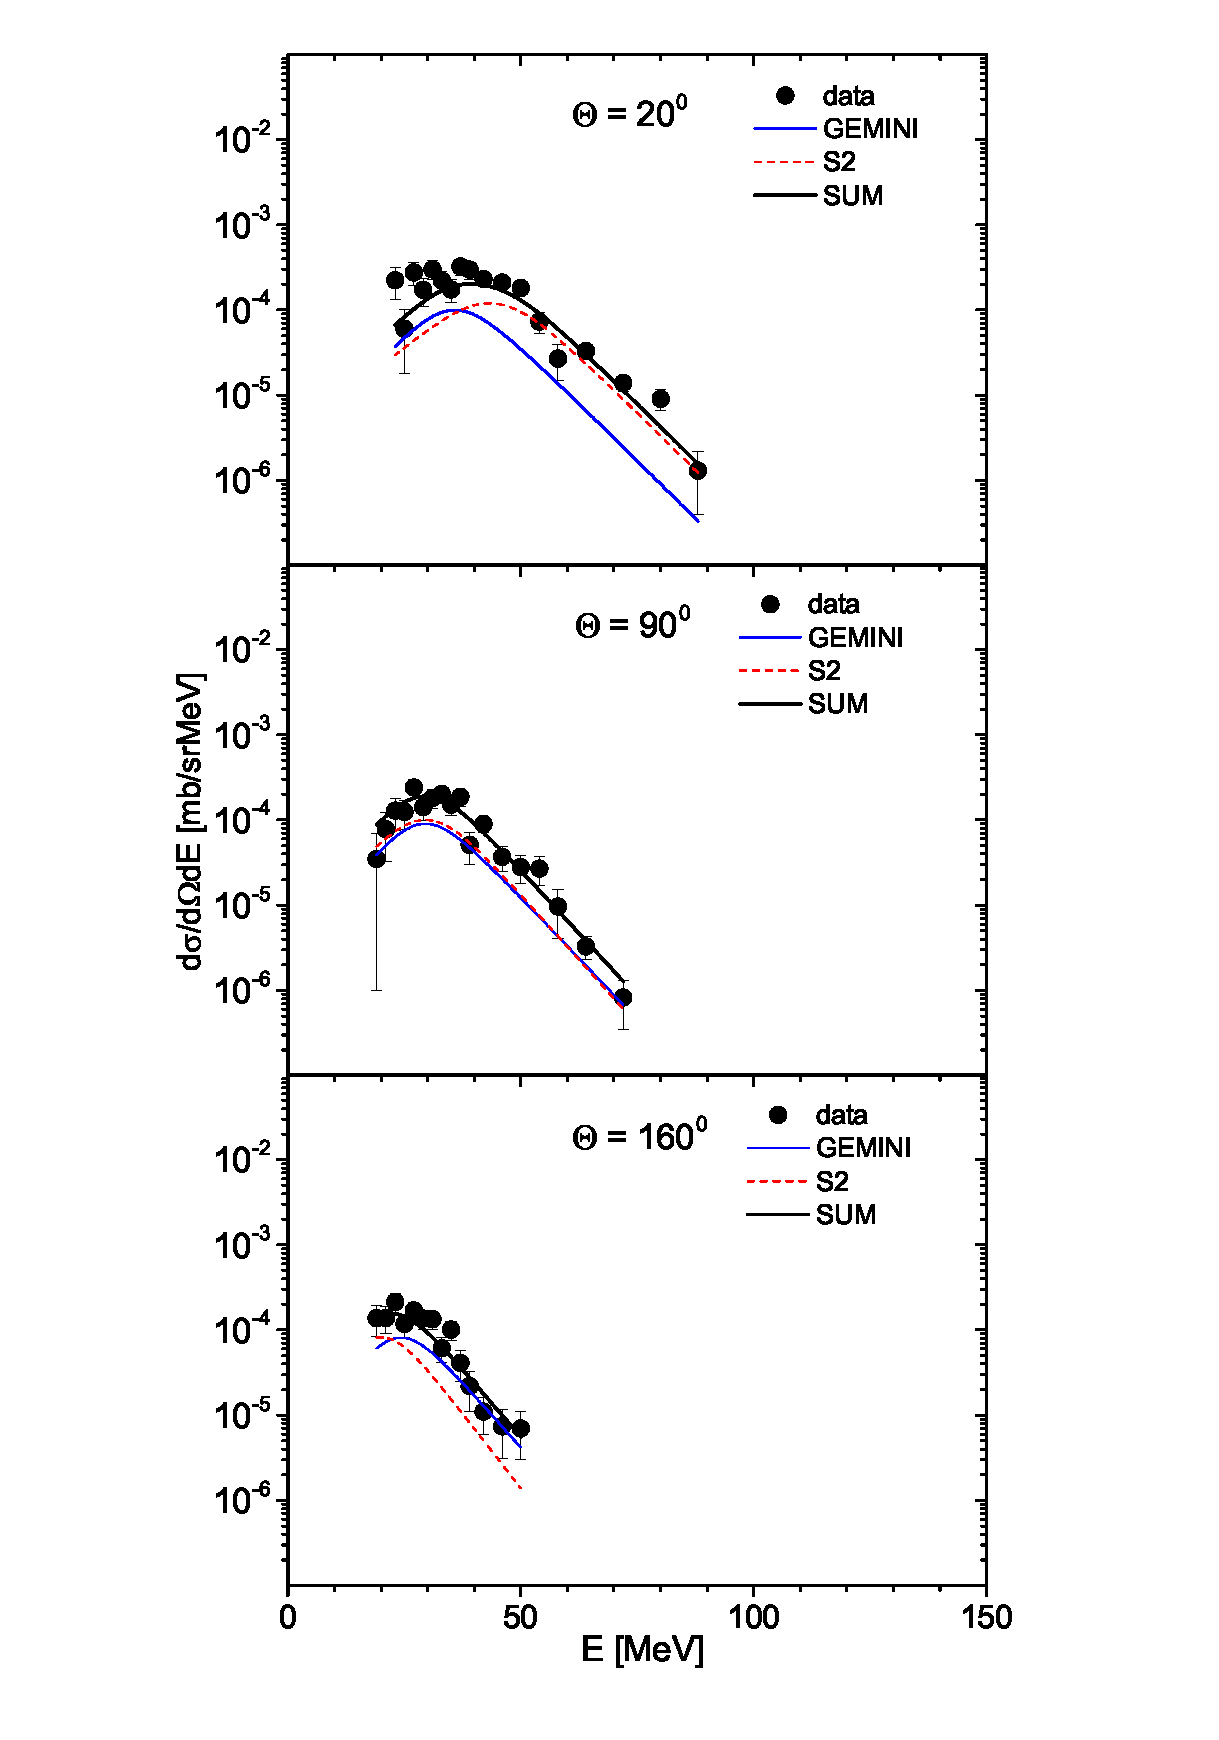
\includegraphics[width=0.65\textwidth]{18OGEMINIS2.eps}
	\caption{Experimental data (dots) and theoretical spectra for $Ag$($p$,$^{18}O$) at three
		scattering angles: 20$^{\circ}$ (top panel), 90 $^{\circ}$ (middle panel) and 120$^{\circ}$ (lower panel).
		The blue (solid) line represents GEMINI++ spectra, the red (dashed) line depicts contribution
		from additional moving source (S2), whereas the black (thick solid) line shows sum of both contributions.}
	\label{fig:18OGEMINIS2}
\end{figure}
%\end{figure*}
%

The source parameters: velocity, an apparent temperature T, its contribution to the total cross-section, and the parameters responsible for the Coulomb barrier that hinders the emission of ejectiles from the source were chosen to reproduce the experimental spectra of the given ejectiles at all scattering angles simultaneously. Details of the moving source model and the interpretation of its parameters can be found in the appendix of Ref. \cite{bubak2007non}.
%\newline 

The data were reproduced very well, with most of the data achieved 
using only one moving source contributions. This is illustrated by fig.~\ref{fig:18OGEMINIS2} in which experimental (filled circles) and model (lines) energy spectra of $^{18}O$ particles are depicted at three scattering angles: 20$^{\circ}$, 90$^{\circ}$ and 160$^{\circ}$.
%
As can be seen, the equilibrium
emission evaluated according to GEMINI++ \cite{CHARITY1988,Charity2010} coupled to
INCL++ \cite{INCLMancusi2014} model (solid, blue line) gives practically
isotropic contribution whereas the non-equilib\-rium emission
represented by single moving source (dashed, red line) dominates at
forward scattering angles but it is much smaller than equilibrium
cross-sections at backward angles. The sum of both contributions
(solid, black line) satisfactorily well reproduces the data.

Only the 10 lightest IMF among all 39 studied particles, \emph{i.e.},
$^{6,7}Li$, $^{7,9,10}Be$, $^{10,11,12}B$ and $^{11,12}C$ needed
application of two moving sources for the good reproduction of
energy spectra at all investigated scattering angles from
20$^{\circ}$ to 160$^{\circ}$.  An example of obtained quality of
the data reproduction is presented in fig.  \ref{fig:9BeGEMINIS2S3}
where the energy spectra of $^9Be$ emitted at the same scattering
angles as in fig. \ref{fig:18OGEMINIS2}, i.e.,  20$^{\circ}$, 90$^{\circ}$ and 160$^{\circ}$ are shown.  

\begin{figure}[!h]
	% Requires \usepackage{graphicx}
	\centering
		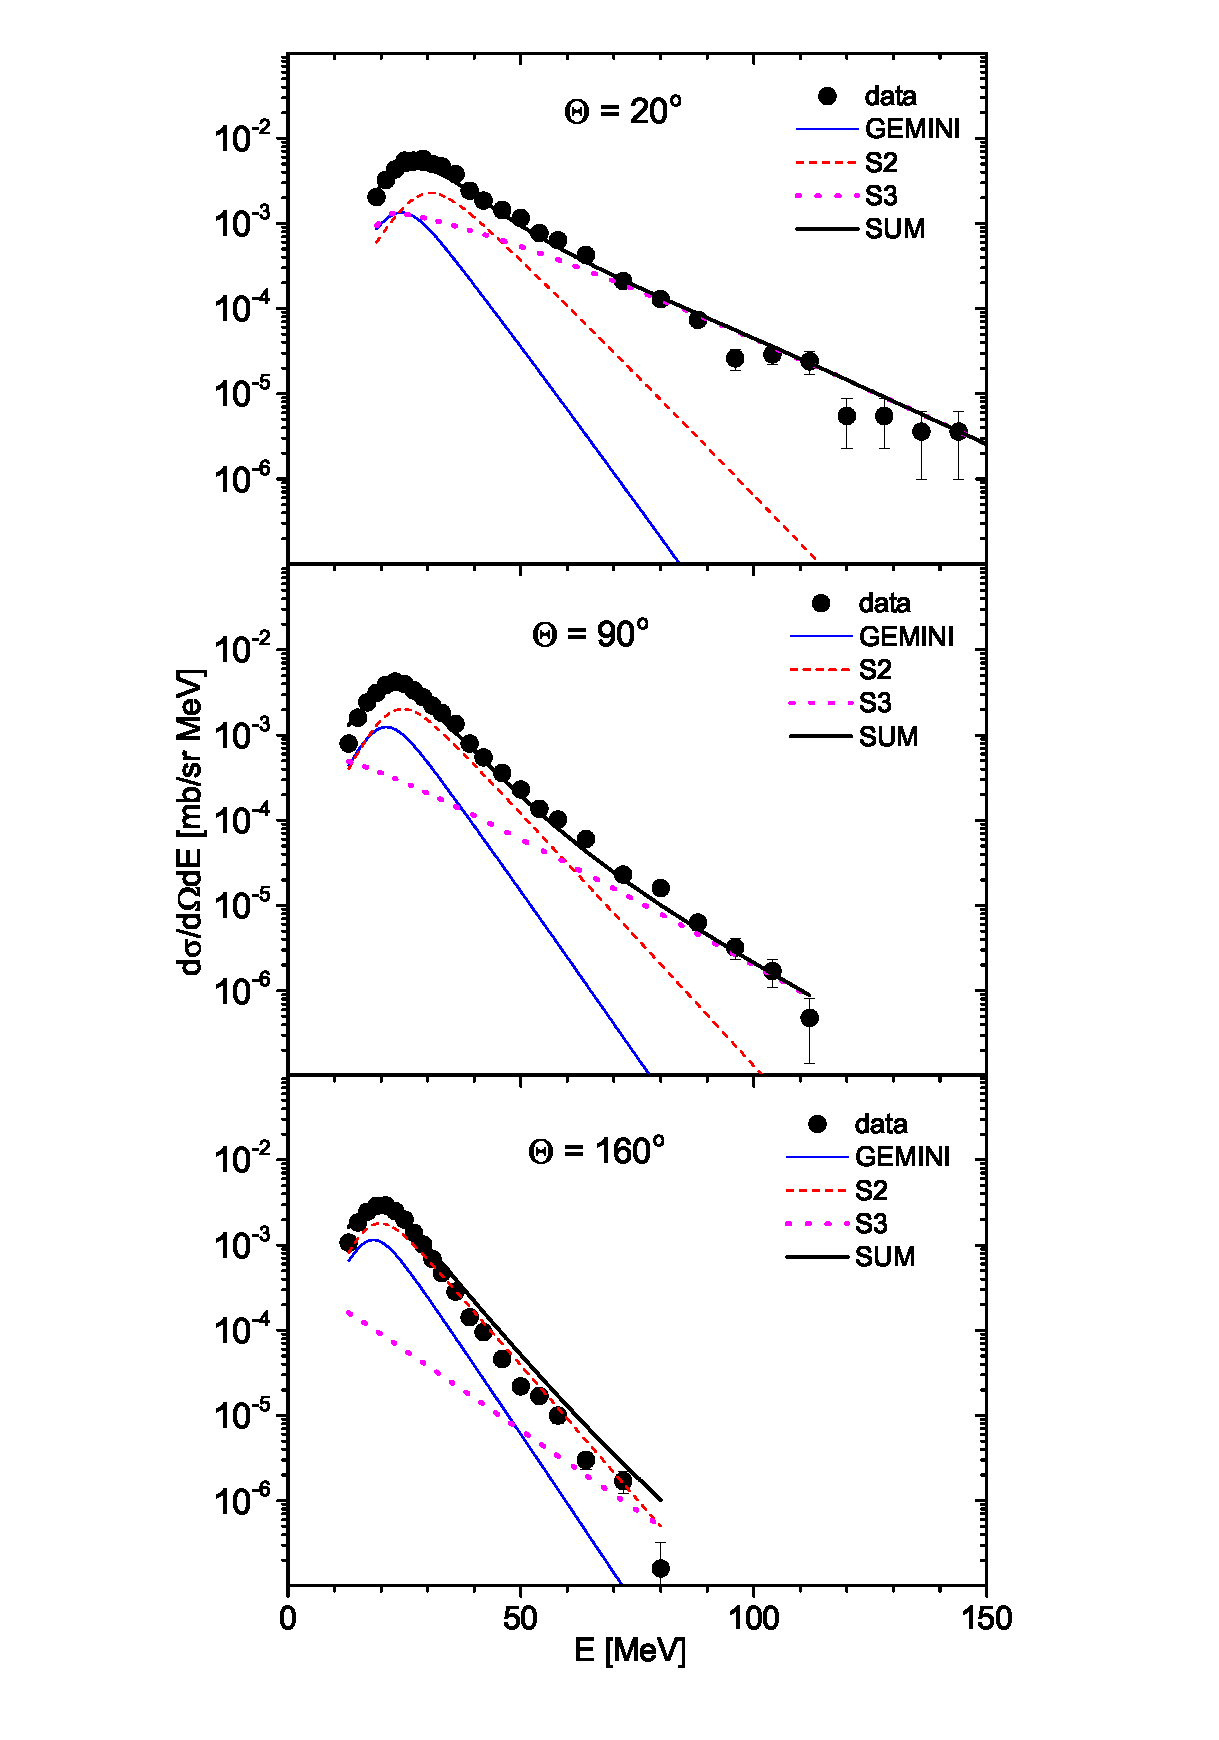
\includegraphics[width=0.6\textwidth]{9BeGEMINIS2S3.eps}
	\caption{Experimental data (dots) and theoretical spectra for $Ag$($p$,$^{9}Be$) at three
		scattering angles: 20$^{\circ}$ (top panel), 90$^{\circ}$ (middle panel) and 120$^{\circ}$ (lower panel).
		The blue (solid) line represents GEMINI++ spectra, the red (dashed) line depicts contribution
		from slower moving source (S2), the magenta (dotted) line shows contribution of the second, faster
		source (S3) whereas the black (thick solid) line shows sum of all contributions.}
	\label{fig:9BeGEMINIS2S3}
\end{figure}
%\end{figure*}

The equilibrium emission
contribution represented by solid, blue line is in this case
significantly smaller than the data for all scattering angles. For
forward scattering angle and small energies the slower of both
moving sources gives dominating contribution - shown as a dashed,
red line - whereas the contribution of faster of the moving sources
- depicted as a dotted, magenta line - reproduces the high energy
tail of the spectrum.  

The situation is different for large
scattering angle where the slower moving source dominates again for
small energies but it gives comparable to the faster source
contribution to the cross-section at high energies.  This is a
typical situation for all analyzed spectra for which introduction of
two moving sources was necessary.
%

The procedure described above enables to obtain the non-equilibrium
production cross-section of IMF equal to the parameter $\sigma_2$ of
the slow moving source (or to the sum of $\sigma_2$ and $\sigma_3$ -
the appropriate parameters of both moving sources).  Furthermore,
sum of the equilibrium production cross-section evaluated by means
of GEMINI++ and the above non-equilibrium cross-section provided
value of the total production cross-section.

The total cross-sections due to INCL++ \cite{INCLMancusi2014} coupled to
GEMINI++ \cite{CHARITY1988,Charity2010} as well as the total cross-sections
obtained by fit of moving sources are presented together in fig. \ref{fig:SGS2S3} as a function of the atomic mass number of
ejectiles. In the lower panel of the figure the equilibrium emission
cross-sections $\sigma_{\text{GEMINI}}$ are shown. In the middle
panel the non-equilibrium cross-sections parameterized by slower of
the moving sources $\sigma_2$ are depicted, whereas that due to the
faster moving source $\sigma_{3}$ are shown in the upper panel of
the figure.  The cross-sections for individual elements are
presented by the same symbols and are connected by lines.
%
%\begin{figure*}[H]
\begin{figure}[!h]
	% Requires \usepackage{graphicx}
	\centering
		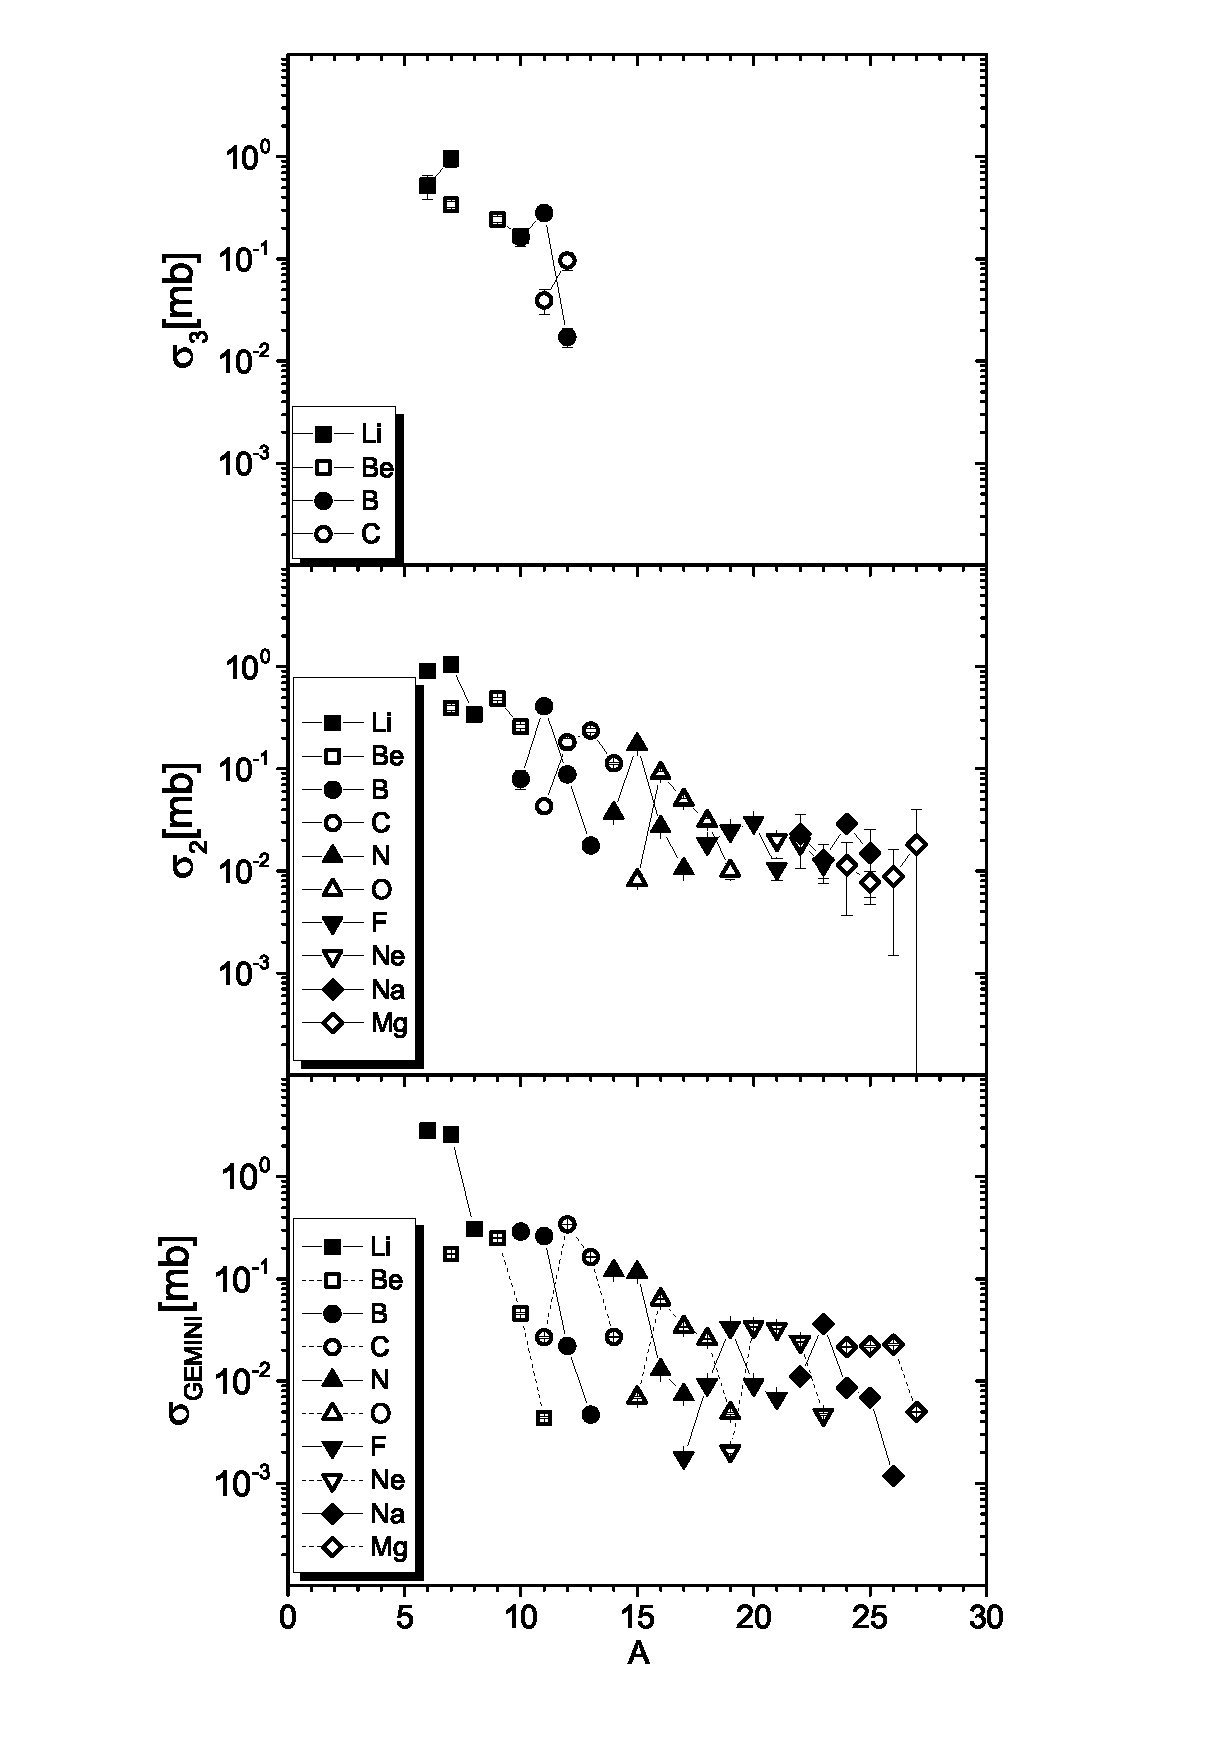
\includegraphics[width=0.63\textwidth]{SGS2S3.eps}
	\caption{Production cross-sections of intermediate mass fragments evaluated by means of
		the INCL++ model coupled to the GEMINI++ one (lower panel),
		production cross-sections $\sigma_2$ from the phenomenological slow moving source (middle panel) and those
		($\sigma_3$) due to the fast moving source (upper panel).  Different elements are distinguished
		by using different symbols whereas  various isotopes
		of the same element are represented by the same symbol.}
	\label{fig:SGS2S3}
\end{figure}
%\end{figure*}
%

It is clear that the cross-sections decrease in average as a
function of the atomic mass number, however, this dependence of the
cross-sections is non-monotonic, parabola - like  for each
individual element. 
%%%
%%%

\section{Ratio of $\sigma_{\text{NEQ}}/\sigma_{\text{TOT}}$ as a function of atomic mass number A}
It is important to note that the mass number A
of the maximal cross-section  determined by the INCL+GEMINI model
for given element is not always the same as the mass number A at
which the maximal cross-section of the non-equilibrium emission
appears. Furthermore, variation of the equilibrium cross-sections
with the mass number seems to be more rapid than variation of the
corresponding non-equilibrium cross-sections. 

Therefore it is quite
difficult to predict 
%from this figure 
how complicated may be the
mass dependence of the ratio of non-equilibrium cross-sections to
the total production cross-sections
$\sigma_{\text{NEQ}}/\sigma_{\text{TOT}}$, i.e.  %\emph{i.e.}, 
 to the sum 
of the equilibrium and non-equilibrium cross-sections.
%
%\vspace{-0.55cm}
\begin{figure}[!h]
	%\begin{figure}[H]
	% Requires \usepackage{graphicx}
	\centering
		\includegraphics*[width=0.98\textwidth]{RNEQtoTOTtot.eps}
	\caption{Atomic mass number A dependence of the ratio of non-equilibrium production
		cross-section  to the total production cross-section for intermediate mass fragments
		emerging from $p+Ag$ collisions.
	}
	\label{fig:RNEQtoTOTtot.eps}
	%\end{figure}
\end{figure}
%
%

The quantified values of the ratios are shown in Fig. \ref{fig:RNEQtoTOTtot.eps} as a function of the atomic mass number A of produced IMF. Different symbols connected by thin lines indicate the values of the ratio for the corresponding elements listed in the description on the right side of the figure.
%

The same symbol depicts  results obtained for various isotopes of a given element. The horizontal line placed at 0.5 value of the ratio
divides  the set of all isotopes into two groups: one with  the
ratio corresponding to the dominance of the equilibrium processes
and the second of the opposite property.
%

The following properties of the ratio of the non-equilib\-rium cross
sections to the total cross-sections may be easily
derived from this figure: 
\begin{itemize}
\item The ratios larger than 0.5 are about 2 times more abundant
than those smaller than 0.5.  This is true for both small and large values of the atomic mass number A.

%
\item Values of  ratios close to 0.5 appear mainly at average
mass number values (A $\sim$ 17) whereas those at smaller as well
as at larger mass numbers are grouped into two separate sets.
One set of the isotopes with the ratios smaller than 0.5
and the second set with the ratios larger than 0.5 for the same A values.
\end{itemize}
Such a specific dependence of the ratio
$\sigma_{\text{NEQ}}/\sigma_{\text{TOT}}$ indicates that there
exists no single monotonic trend of this ratio versus mass number A
for all studied isotopes. One has to find some additional criterion
which might select the isotopes into groups behaving in the same way
when treated as a function of the mass number.Two specific properties of the emitted intermediate mass fragments were applied
for this purpose:

(i) the even/odd number of protons and neutrons - constituents of
the IMF, and

(ii) the third component of the isospin of the fragment T$_3 \equiv
(N-Z)/2$ representing excess (deficiency) of the number of neutrons
in respect to the number of protons. For this purpose all reaction
products were divided into 4 subgroups of definite (Z,N): (even -
even), (even - odd), (odd - even) and (odd - odd). The atomic mass
dependence of the ratio $\sigma_{\text{NEQ}}/\sigma_{\text{TOT}}$
was presented for these subgroups in separate panels of the Fig.
\ref{fig:R4eoT3}; the upper-left panel for even-even (Z,N), the
upper-right one for even-odd, \emph{etc.}, in the clockwise
direction.

It turned out that the ratio
$\sigma_{\text{NEQ}}/\sigma_{\text{TOT}}$ behaves in a very regular
way for each of these selected groups of isotopes (cf. Fig.
\ref{fig:R4eoT3}). Especially, it may be stated that this ratio
decreases in average linearly with the mass number A of emitted
fragment for even-even, even-odd and odd-even intermediate mass
fragments whereas it increases in average linearly for odd-odd
ejectiles.
%
\begin{figure}[!h]
	\centering
	
		\includegraphics*[width=0.96\textwidth]{R4eoT3.eps}
	\caption{Atomic mass number A dependence of the ratio of non-equilibrium production
		cross-section to the total production cross-section for intermediate mass fragments
		emerging from p+Ag collisions.  % at proton beam energy E$_p$=0.48 GeV.
		Left upper panel of the figure presents the results for even-even (Z,N) products
		whereas other panels
		(in clockwise direction) contain results for even-odd, odd-even and odd-odd products.
		Different symbols are attributed to values of the ratio corresponding to different values of the third
		component of the isospin $T_3=(N-Z)/A$ of ejectiles. Dashed lines are drawn to guide the eye.}
	\label{fig:R4eoT3}
	%\end{figure}
\end{figure}
%
Furthermore, some deviations from such a regular behaviour may be
observed for specific values of the third component of the isospin
$T_3 \equiv (N-Z)/2$ of the emitted particles. For example, two of
the four even-even ejectiles with $T_3=0$, namely $^{12}$C and
$^{20}$Ne have much smaller ratio
$\sigma_{\text{NEQ}}/\sigma_{\text{TOT}}$ than other even-even IMF
with $T_3=0$ and all $T_3=1$ particles 
(cf. upper, left panel of Fig. \ref{fig:R4eoT3}).
%\vspace{-0.3cm}

Second of such
deviations is the fact that all $T_3=3/2$ nuclides for even-odd and
odd-even ejectiles have larger
$\sigma_{\text{NEQ}}/\sigma_{\text{TOT}}$ ratio than that which
characterizes the $T_3=-1/2$ and $T_3=1/2$ nuclides (cf. upper-right
and lower-right panel of the Fig. \ref{fig:R4eoT3}).

The third example consists in the systematic deviation toward
smaller ratio values of $T_3=0$ ejectiles in respect to the straight
line averaging behaviour of the odd-odd group of ejectiles whereas
the IMF with $T_3=1$ deviate toward larger ratio values (cf.
lower-left panel of the Fig. \ref{fig:R4eoT3}).
%
%
\vspace{-0.3cm}
\begin{figure}[!h]
	%%\begin{figure}[H]
	% Requires \usepackage{graphicx}
	\centering
	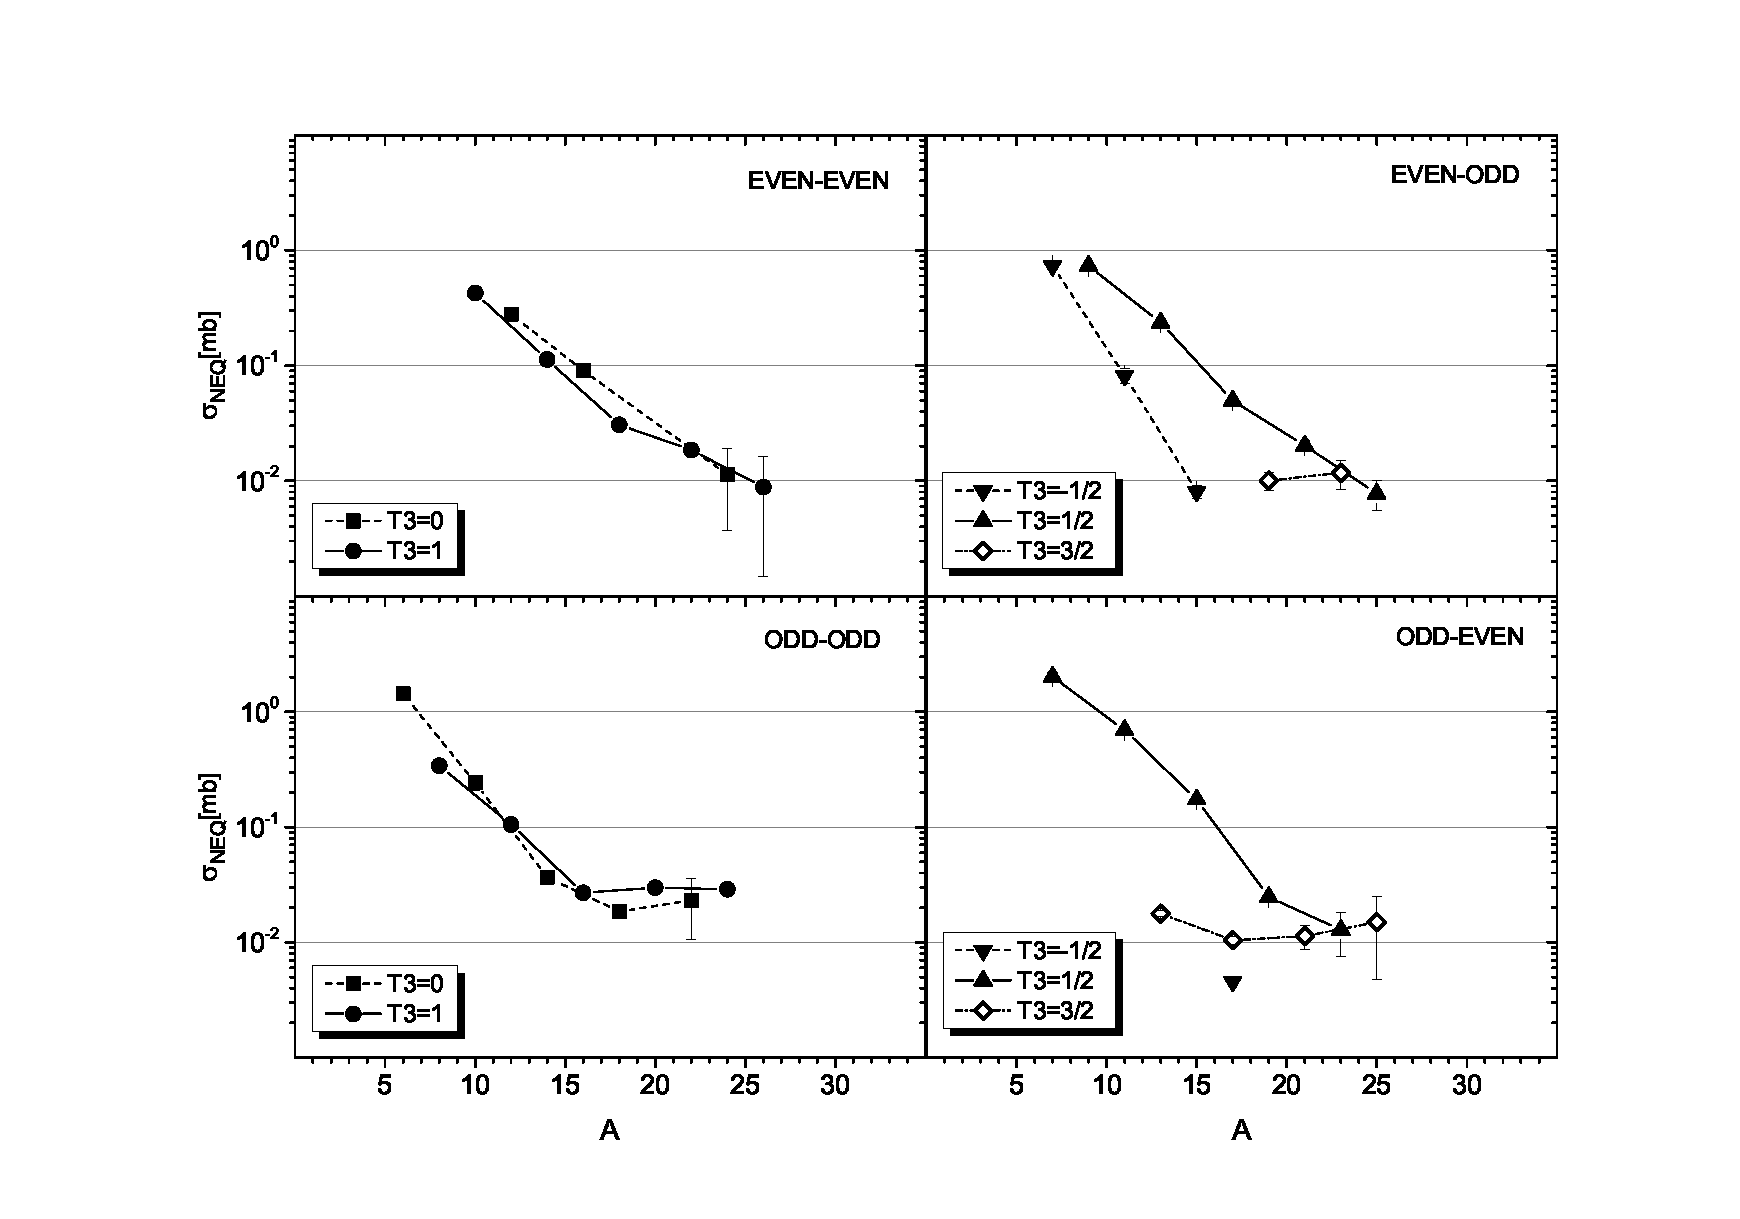
\includegraphics[width=0.88\textwidth]{S23vsAT3.eps}
	\caption{Atomic mass number dependence of  the production
		cross-sections of intermediate mass fragments
		emerging due to non-equilibrium processes from p+Ag collisions.   Left upper panel
		of the figure presents the results for even-even (Z,N) products whereas other panels
		(in clockwise direction) contain results for even-odd, odd-even and odd-odd products.
		Different symbols are attributed to values of the cross-sections for fragments with different values of the third
		component of the isospin $T_3=(N-Z)/A$. The solid, dashed and dot-dashed lines are drawn to guide the eye.}
	\label{fig:S23vsAT3}
	%%\end{figure}
\end{figure}
While no physical model has been implied by the dependence presented
in the Fig. \ref{fig:R4eoT3}, the extremely regular behaviour
achieved in this  analysis certainly merits further consideration. The above regular variation of the $\sigma_{\text{NEQ}}/\sigma_{\text{TOT}}$ ratio indicates that the total cross-sections as well as the cross-section of equilibrium and non-equilibrium processes must behave in a regular way for the selected groups of IMF.
%
\vspace{-0.3cm}
\begin{figure}[!h]
	%%\begin{figure}[H]
	% Requires \usepackage{graphicx}
	\centering
		\includegraphics*[width=0.88\textwidth]{TOTG23T3.eps}
	\caption{The same as in Fig. \ref{fig:S23vsAT3} but for the total
		production cross-sections, \emph{i.e.}, for the sum of equilibrium and non-equilibrium production cross-sections.
		The solid, dashed and dot-dashed lines are drawn to guide the eye.
	}
	\label{fig:TOTG23T3}
	%%\end{figure}
\end{figure}
%
%\vspace{-0.4cm}
\begin{figure}[!h]
	\centering
	\includegraphics*[width=0.88\textwidth]{GEMseparateT3.eps}

	\caption{The same as in Fig. \ref{fig:S23vsAT3} but for the equilibrium
		emission cross-sections evaluated by means of the INCL++ plus GEMINI++
		models. The solid, dashed and dot-dashed lines are drawn to guide the eye.
	}
	\label{fig:GEMseparateT3}
	%%\end{figure}
\end{figure}
%
  To check the above statement the mass number dependences  of the cross-sections for even-even, even-odd,\emph{ etc.}, reaction products are depicted in four panels (ordered in the same manner as in Fig. \ref{fig:R4eoT3}) of Figs. \ref{fig:S23vsAT3}, \ref{fig:TOTG23T3} and \ref{fig:GEMseparateT3} for pre-equilibrium processes, for sum of pre-equilibrium and equilibrium processes and for equilibrium emission, respectively.
As can be seen,  the production cross-sections  of different mechanisms behave in very similar manner, when the group of even-odd or odd-even  fragments is taken into consideration (cf. right-upper and right-lower panels of Figs.  \ref{fig:S23vsAT3}, \ref{fig:TOTG23T3} and \ref{fig:GEMseparateT3}). Three well separated groups of the cross-sections are visible
corresponding to T$_3=-1/2$, T$_3=1/2$, and T$_3=3/2$. Those representing particles with T$_3=-1/2$ and T$_3$=1/2 show fast, exponential decreasing of the cross-sections versus the mass number A whereas the cross-sections of products with T$_3$=3/2 are almost independent of the mass number.  It should be also noted that the decreasing of the cross-sections for particles with T$_3=-1/2$ is much faster than that for particles with T$_3$=1/2.
  
  
  The situation for even-even and odd-odd particles is different  in respect to
  that described above
(cf. left-upper and left-lower panels of
  Figs. \ref{fig:S23vsAT3}, \ref{fig:TOTG23T3} and \ref{fig:GEMseparateT3}).
  The mass dependence of the cross-sections for particles with
  T$_3=0$  and T$_3=1$ does not differ as strongly as that of the cross-sections
  for fragments
  with T$_3=-1/2$, T$_3$=1/2 and T$_3$=3/2, however, this difference changes from mechanism
  to mechanism.  For non-equilibrium processes (cf. left-upper and left-lower panels of Fig.
  \ref{fig:S23vsAT3}) the difference is almost negligible.  It
  increases for total cross-sections (cf. corresponding panels of
  Fig. \ref{fig:TOTG23T3}) and becomes quite significant for equilibrium
  cross-sections (cf. Fig. \ref{fig:GEMseparateT3}).
%
